\documentclass[8pt]{article}

\usepackage[utf8]{inputenc}
\usepackage[ngerman]{babel}
\usepackage{amsmath}
\usepackage{nicefrac}
\usepackage{color}
\usepackage[hidelinks]{hyperref}
\usepackage{graphicx}
\usepackage{stmaryrd}
\usepackage[a4paper,top=2cm,left=4cm,right=4cm,bottom=2cm,marginparwidth=5cm]{geometry}
\usepackage{marginnote}
\usepackage[automark]{scrpage2}
% Externe PDF's einbinden können
\usepackage{pdflscape}
\usepackage[final]{pdfpages}
\pagestyle{scrheadings}

\newcommand{\secauthor}[1]{\textbf{Autor(en) dieses Kapitels: {#1}}\\}

\newcommand{\fatnote}[1]{\marginnote{\textbf{#1}}}
\newcommand{\leftnote}[1]{\reversemarginpar\fatnote{#1}}
\newcommand{\rightnote}[1]{\normalmarginpar\fatnote{#1}}

\newcommand{\defin}[1]{\noindent #1\vspace{0.3cm}}
\newcommand{\ldefin}[2]{\leftnote{#1}\defin{#2}}
\newcommand{\rdefin}[2]{\rightnote{#1}\defin{#2}}

\newcommand{\todo}[1]{\textcolor{red}{\textbf{TODO}: #1}}

\newcommand{\coursename}{\@empty}
\newcommand{\groupno}{\@empty}

\newcommand{\course}[2]{\renewcommand{\coursename}{#1}\renewcommand{\groupno}{#2}}
\newcommand{\beginsheet}{\clearscrheadfoot\ihead[]{Kurs: \coursename}\ohead[]{Gruppe \groupno}\ofoot[]{\pagemark}\ifoot[]{}}

\newcommand{\email}[1]{\href{mailto:#1}{#1}}


%%%%%%%%%%%%%%%%%%%%%%%%%%%%%%%%%%%%%%%%%%%%%%%%%%%%%%%%%%%%%%%%%%%%%%%%%%%%%%%%%%%%%%
%% Oberhalb dieses Blocks nichts ändern
%%%%%%%%%%%%%%%%%%%%%%%%%%%%%%%%%%%%%%%%%%%%%%%%%%%%%%%%%%%%%%%%%%%%%%%%%%%%%%%%%%%%%%


%% TODO: Hier die fehlende Gruppennummer einfügen
\course{Lisp Kurs -- Roboterprogrammierung in Lisp}{4}


\begin{document}

\beginsheet

\title{SUTURObot}
\author{Jannik Buckelo, Simon Stelter\\ 
\texttt{jannikbu@tzi.de, stelter@tzi.de}}
\date{13.07.2014}
\maketitle

%\newpage

%\tableofcontents

%\newpage

\begin{abstract}
Dokumentation des SUTURObots der im Rahmen des Lisp Tutorials an der Universit"at Bremen erstellt wurde. Zur Konstruktion des Roboters wurde ein LEGO Mindstorm verwendet, der mittels eines Smartphones gesteurt werden kann. Die Steuerung der Motoren und das Auswerten der Sensoren wird dabei von einem Common Lisp-Programm geregelt.	
\end{abstract}

\section{Einleitung} 
\secauthor{Simon}
Im Rahmen eines Lisp Tutorials haben wir mit LEGO Mindstorm Roboter gebaut und dann mit Lisp gesteuert. Es wurde als erstes der SUTURObot v1 (siehe Abb. \ref{fig:SUTURObot1}) gebaut, dieser sollte auf zwei parallel ausgerichteten Rädern balancieren können. Für die Bestimmung der Lage sollte ein Smartphone verwendet werden, welches mit einer Android-App die Lage des Handy's ausliest und an das Lisp programm zur verarbeitung sendet.\\
Da die Daten des selbst gebaut Sensors für dieses Vorhaben jedoch zu spät ankamen, wurde der SUTURObot v2 (siehe Abb. \ref{fig:SUTURObot2}) entwickelt. Dieser hat eine holonome Basis und soll mit der vorher entwickelten Android-App frei bewegt werden können. Zusätzlich sollte er auf Kollisionen reagieren können.\\
Der Quellcode ist verfügbar unter \cite{Code}.

\section{SUTURObot v1}
\begin{figure}[h]
  \begin{center}
    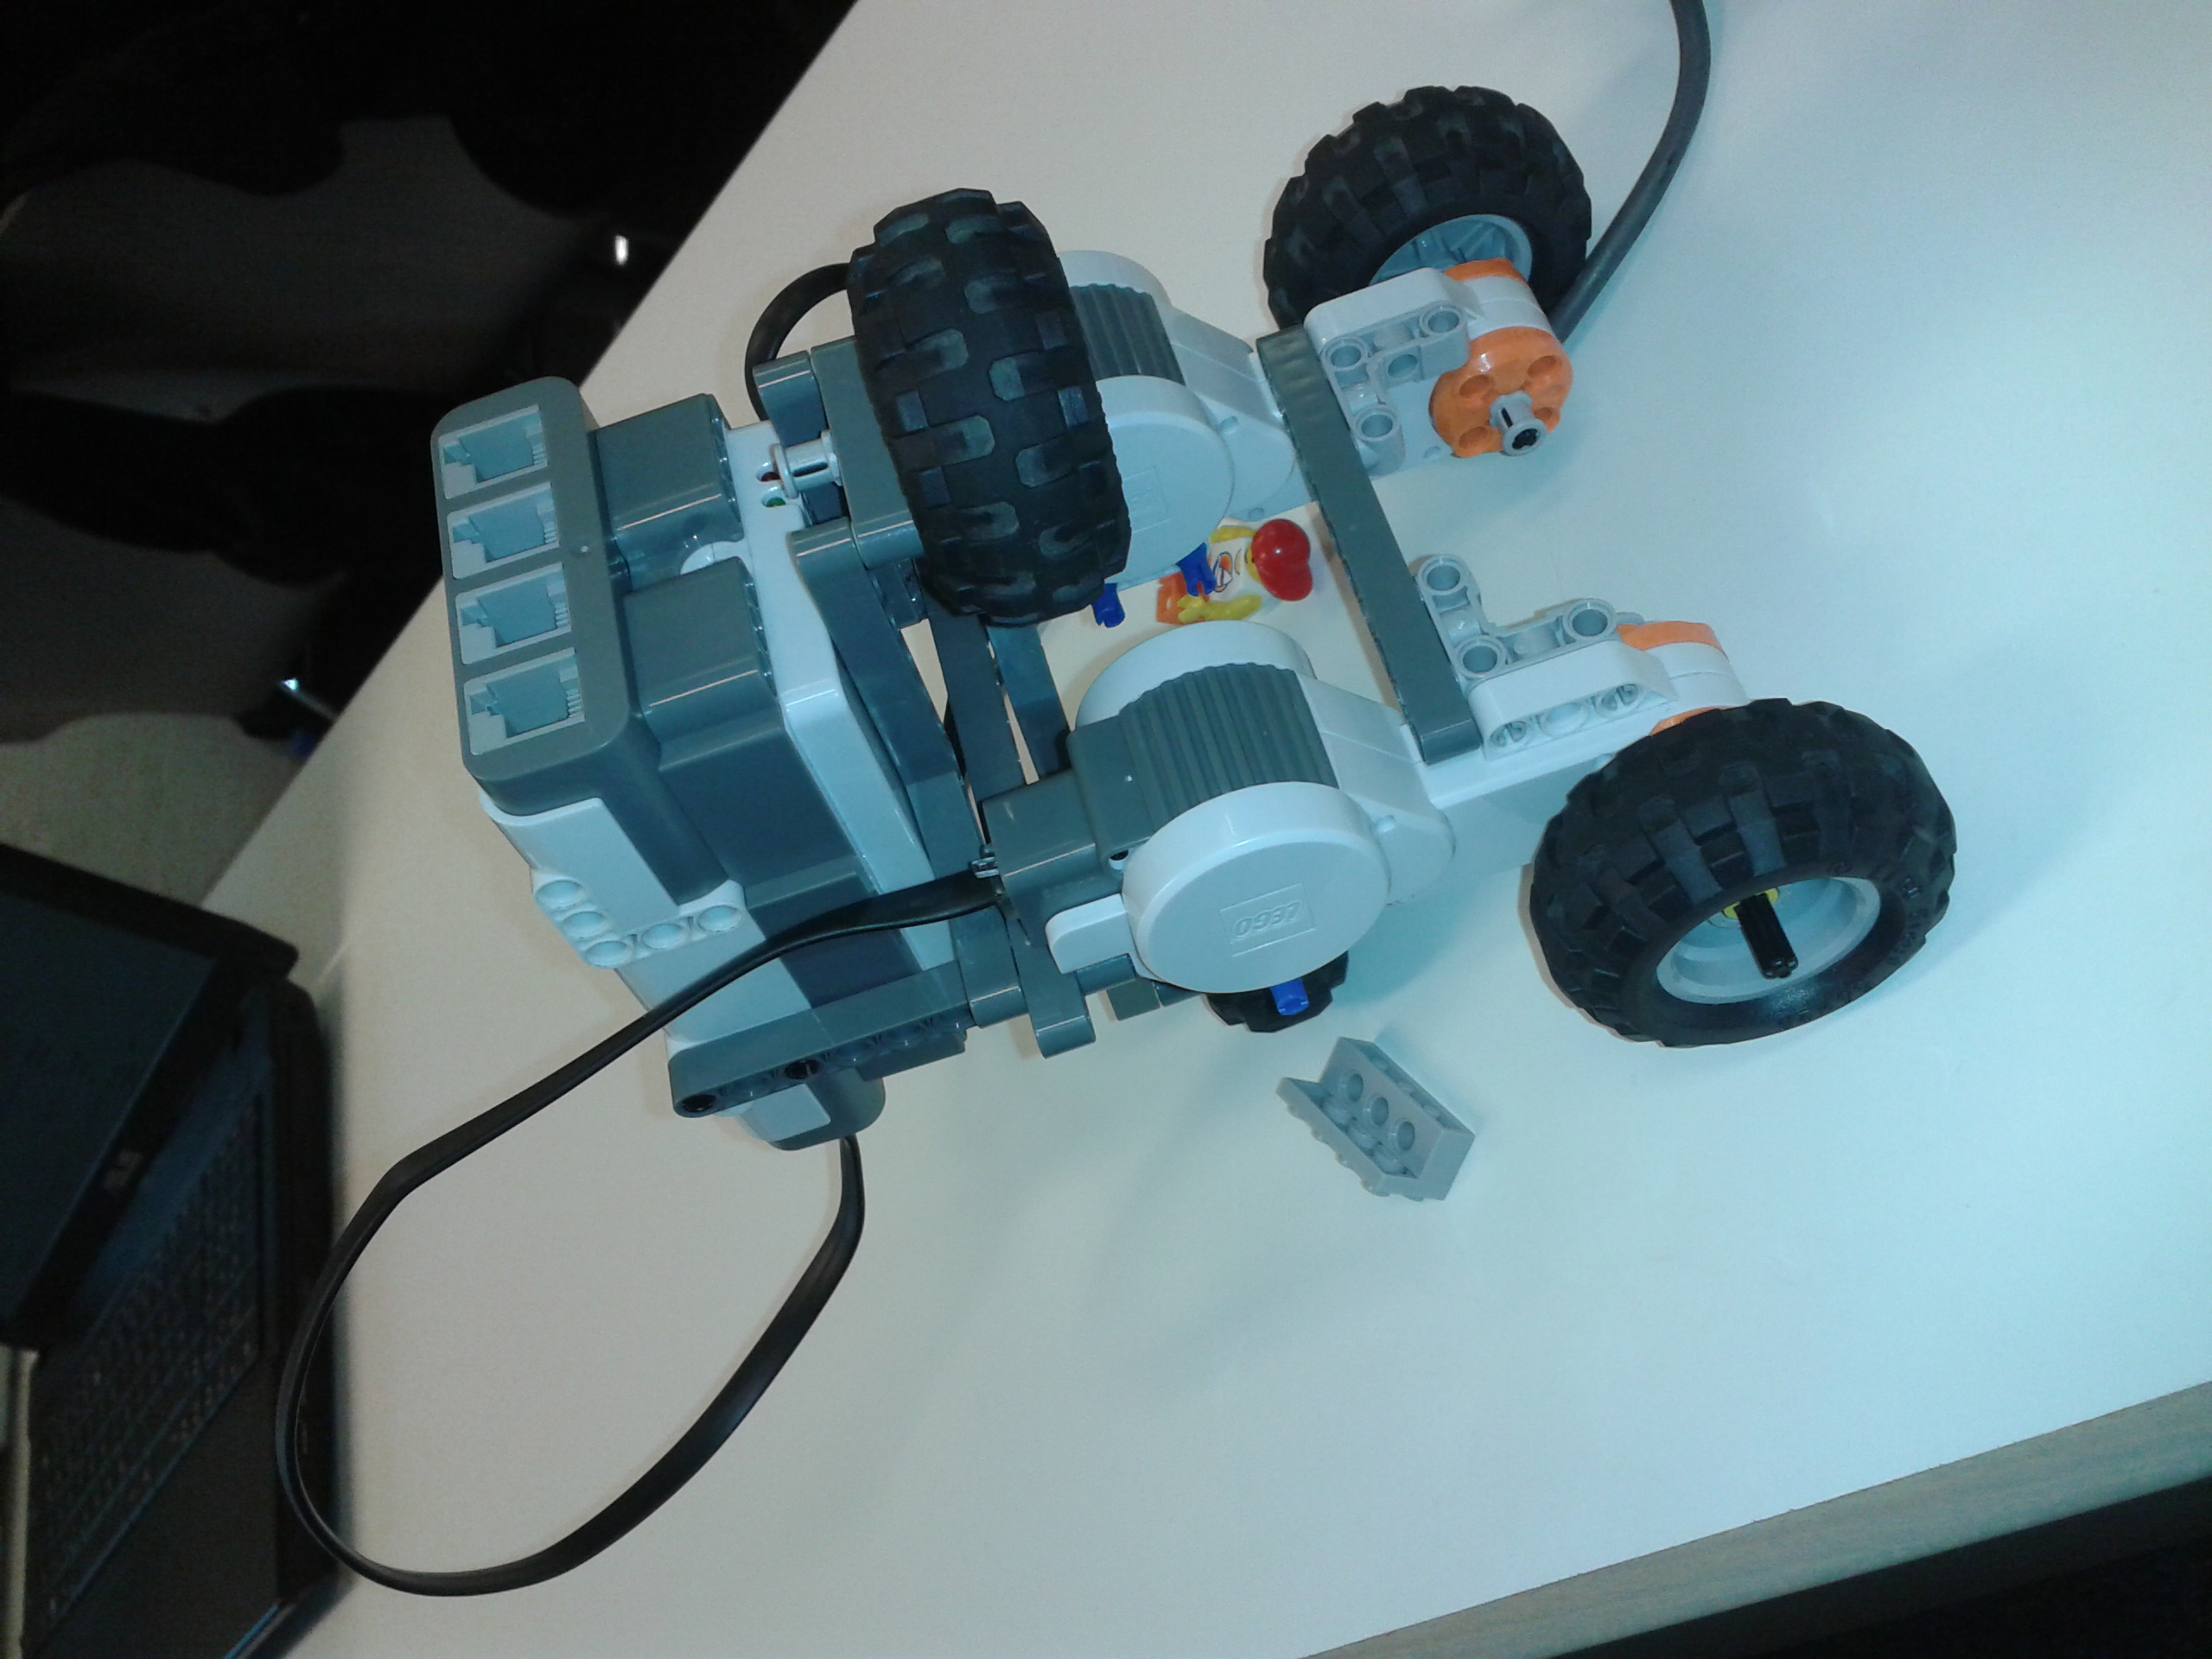
\includegraphics[width=.5\textwidth]{pictures/SUTURObot-v1.jpg}  
  \end{center}
  \caption{SUTURObot v1}
  \label{fig:SUTURObot1}
\end{figure}

\subsection{Idee und Lösungsansatz} 
\secauthor{Simon}
Wir haben uns am Anfang dafür entschieden einen Roboter zu bauen, der auf zwei parallel stehenden Rädern balancieren und fahren kann. Dafür benötigten wir passende Sensor, um die Lage des Roboters zu bestimmen. Da uns kein Gyrosensor von Lego zu Verfügung stand und die Daten aus dem Ultraschallsensor zu stark mit Rauschen belastet waren, haben wir uns dafür entscheiden, den Lagesensor eines Smartphones zu verwenden. Unsere grundlegende Idee war es dann aus der Lage den Fehler zu bestimmen und mit einem PID-Controller die Balance zu halten bzw zu fahren. Von Balancieren sollte zum Fahren gewechselt werden, indem mittels des PID-Controllers eine leicht gekippte Haltung eingenommen wird.

\subsection{Architektur}

\subsubsection{Allgemein} 
\secauthor{Jannik}
In dem Callback des Lagesensors berechnen wir den Fehler unserer momentanen Lage, also die Differenz zwischen der von dem Lagesensor erhaltenen Lage und unserer gew"unschten Lage, und geben diese in einer Liste mit den letzten 10 Fehlern an den PI-Controller. Das Erbgeniss des PI-Controllers geben wir dann als Effort an die Antriebsmotoren und zusammen mit der Lage an die Visualisierung.


\subsubsection{Sensorik} 
\secauthor{Simon}
Um den Lagesensor des Smartphones auszulesen haben wir eine Android-App geschrieben, die den ausgelesenen Quaternion unverändert auf einem topic veröffentlicht.
Für unser Vorhaben war es nötig aus dem Quaternion die Neigung zu bestimmen. Dazu reichte jedoch keine einfache Umrechnung in Eulerwinkel, da zum einen die Lösung nicht eindeutig ist und zum anderen es unter bestimmten Bedingungen überhaupt keine gibt. Wir haben daher die Funktion \texttt{pitch} implementiert um die Neigung zu berechnen. In dieser erstellen wir zwei identische Vektoren, $\left( \begin{array}{c} 1 \\ 0 \\ 0
\end{array} \right)$. Einen davon rotieren wir mit der Quaternion vom Handy. Wenn wir nun den Winkel zwischen beiden bestimmen, erhalten wir die Neigung. Da jedoch mit diesem Verfahren sowohl eine Vorwärts-, als auch eine Rückwärtsneigung einen positiven Winkel liefert, neigen wir den zweiten Vektor vor der Winkelbestimmung um $pi / 2$. Wenn wir dann von der gewonnenen Neigung $pi / 2$ abziehen, kann man zwischen einer Vorwärts- und Rückwärtsneigung anhand des Vorzeichens unterscheiden.

\subsection{Probleme} 
\secauthor{Simon}
Tests mit dem SUTURObot v1 haben ergeben, dass der Lagesensor, das die Daten"ubertragung vom Handy zum Laptop oder die Datenübertragung vom Laptop zum Brick zu viel Zeit in Anspruch nimmt, um mit den Motoren einem Sturz rechtzeitig entgegen wirken zu können. Da uns leider kein weiteres Handy mit den passenden Sensoren zur Verfügung stand, um die erste Fehlerquelle auszuschließen, haben wir uns dafür entschlossen, stattdessen den SUTURObot v2 zu entwickeln.

\section{SUTURObot v2}
\begin{figure}[h]
  \begin{center}
    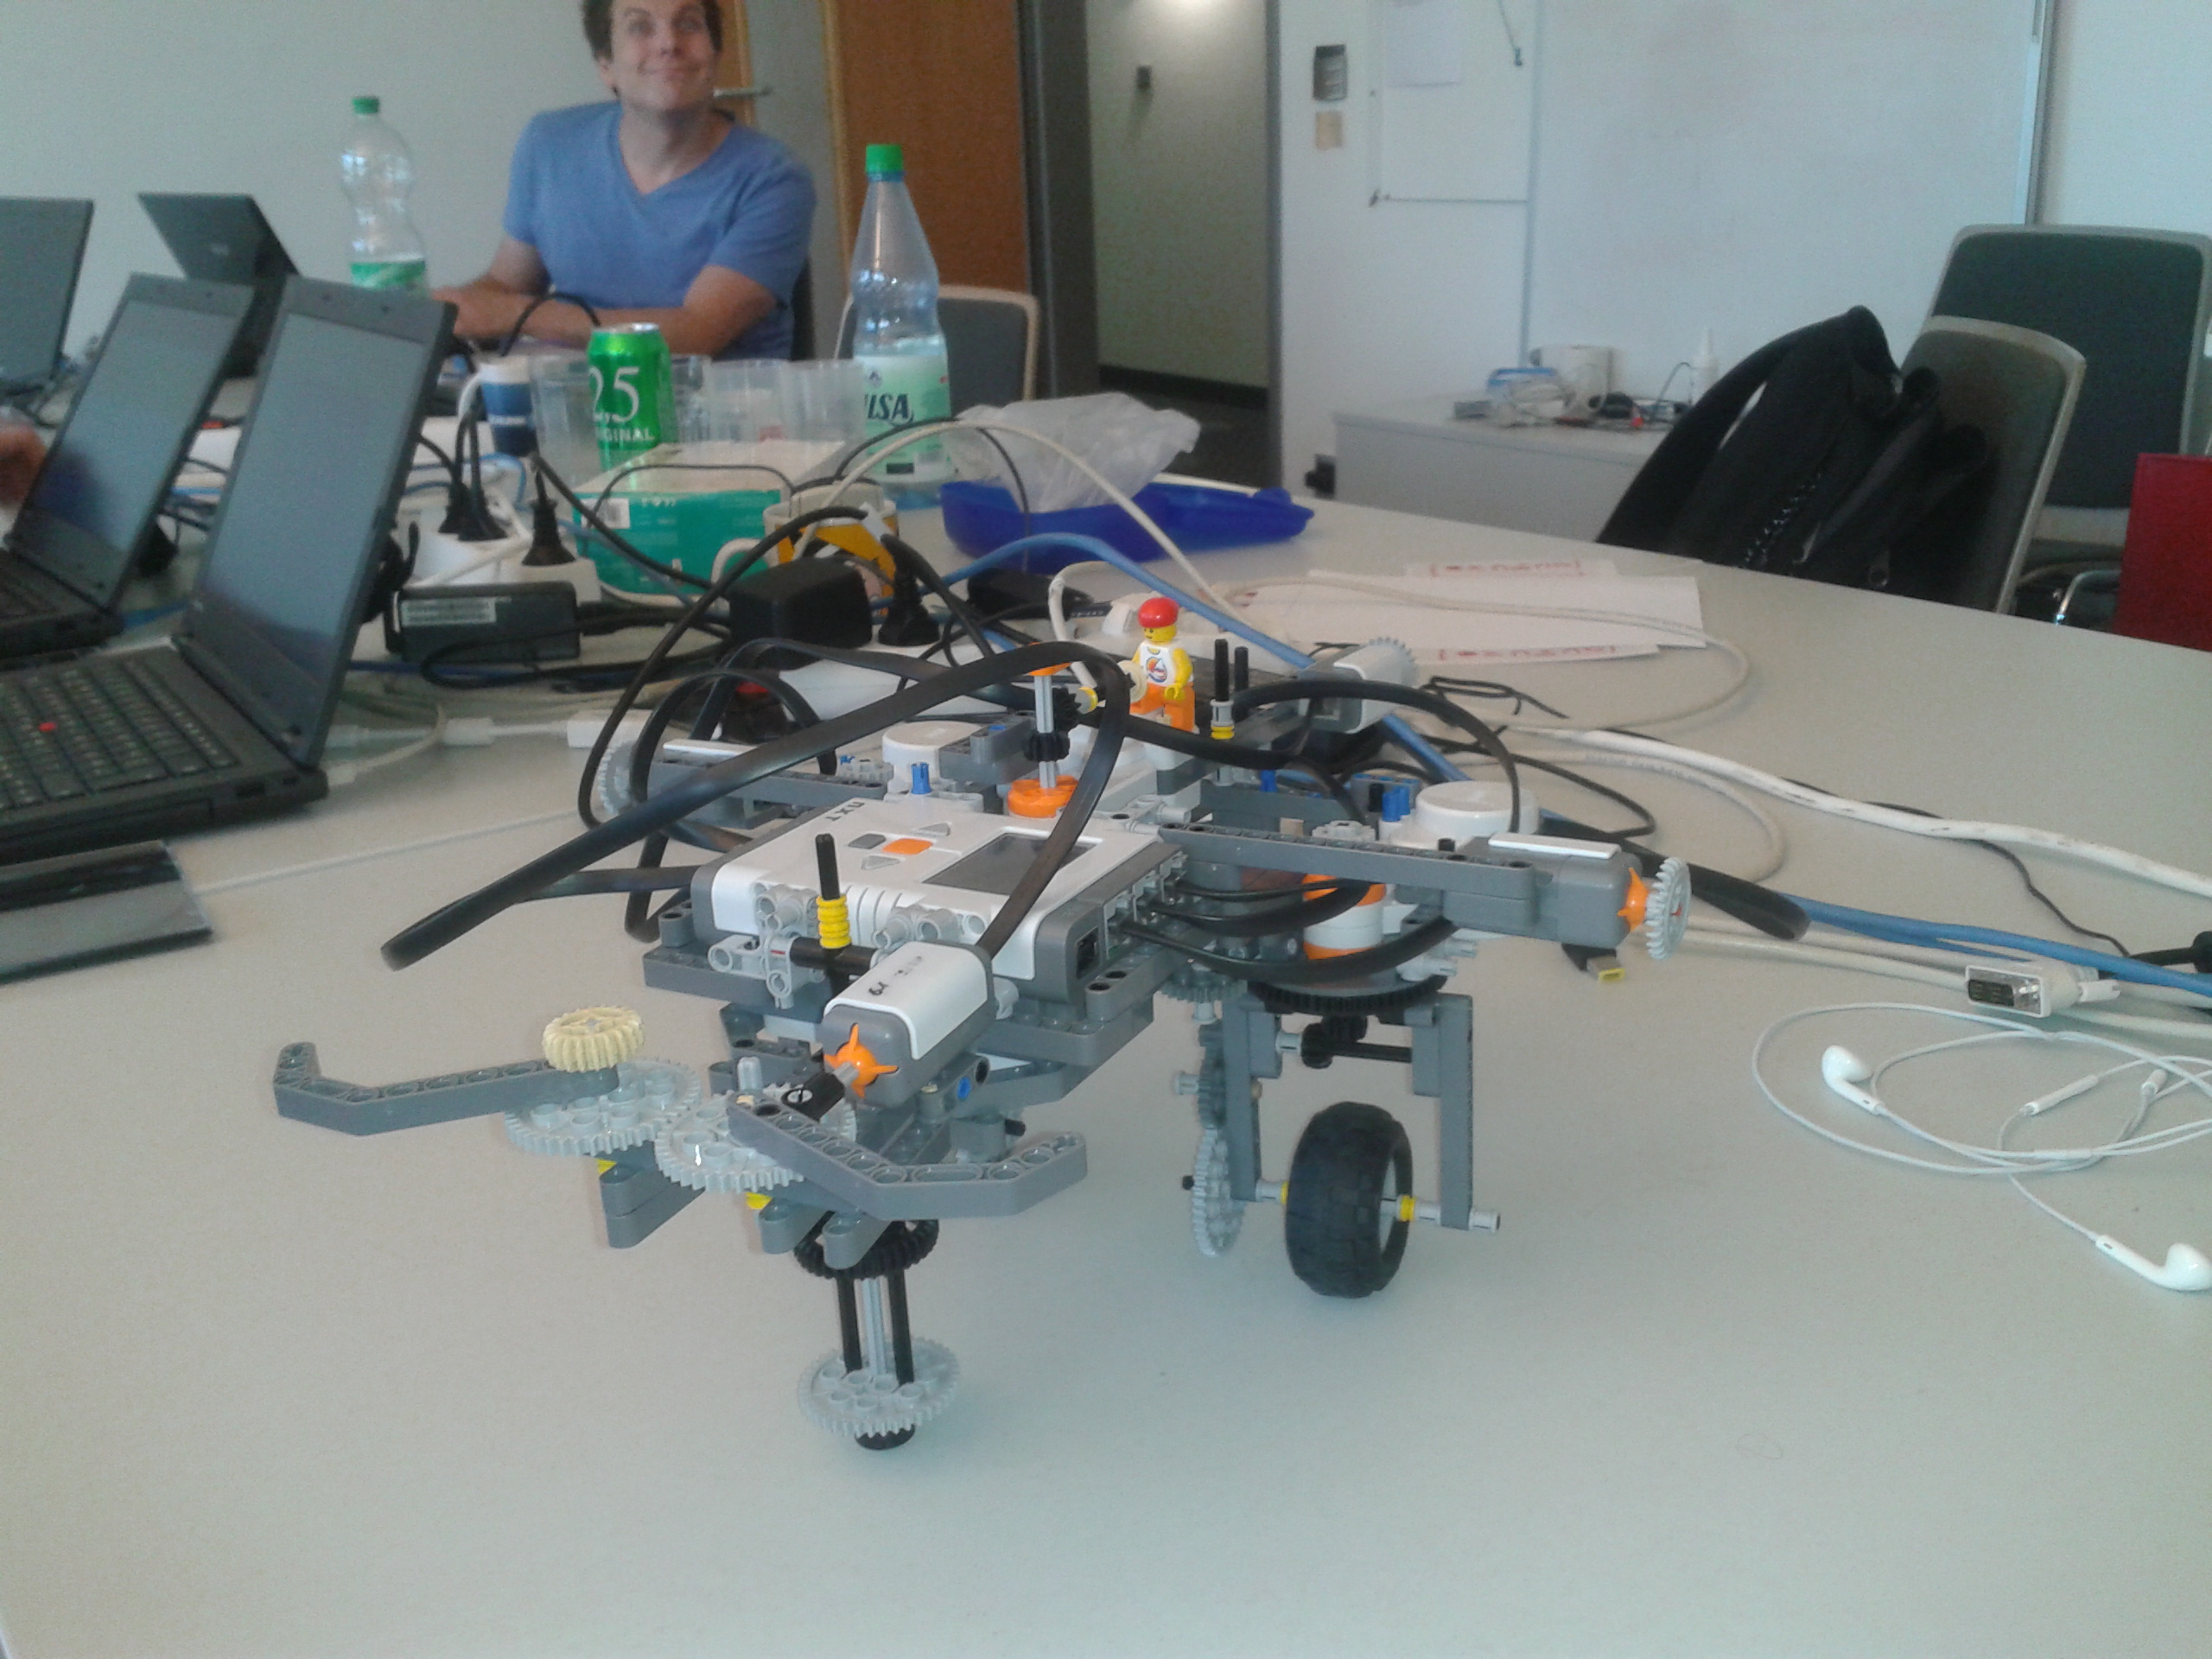
\includegraphics[width=.5\textwidth]{pictures/SUTURObot-v2.jpg}
  \end{center}
  \caption{SUTURObot v2}
  \label{fig:SUTURObot2}
\end{figure}

\subsection{Idee und Lösungsansatz} 
\secauthor{Jannik}
Nachdem unser SUTURObot v1 aus vorher beschriebenen Gr"unden nicht funktionert hat, mussten wir uns ein neues Konzept ausdenken. Wir wollten dabei m"oglichst viel von unserem bis dahin erstellten Code und Infrastruktur wiederverwenden. Also haben wir uns "uberlegt die bereits bestehende Android-App und Funktionen zur Lagebestimmung des Handys zu verwenden, um den Roboter zu steuern.

Wir haben dazu eine holonome Basis f"ur den Roboter gebaut und die App mit zwei zus"atzlichen Buttons ausgestattet, sodass der Effort der R"ader mittels kippen des Smartphones geregelt werden kann und die Drehung der R"ader mittels Buttonklick. Au"serdem haben wir vier Drucksensoren an den Seiten des Roboters zur Erkennung von Kollisionen angebracht. Sollte es zu einer Kollision kommen soll der Roboter selbst"andig die Bewegung in Richtung des Hindernisses einstellen und ein St"uck von dem Hindernis wegfahren.

\subsection{Architektur}

\subsubsection{Allgemein}
\secauthor{Jannik}
In unserem Kontrollprogramm "uberpr"ufen wir in einer Schleife, ob eine Kollision erkannt wurde oder nicht. Wurde keine Kollision erkannt, wird die funktion zur Steuerung des Roboter ausgef"uhrt. Diese berechnet aus der Drehung des Handys um die x-Achse wie stark der Effort auf den Antriebsmotoren sein soll, und aus der Drehung um die y-Achse die Differenz zwischen den Efforts der beiden Motoren. Unterschreitet der Effort den Mindestwert, der ben"otigt ist zum Antreiben der Motoren, wird keine Effort an die Motoren gegeben. Die Drehung um die y-Achse erfordert ebenfalls einen Mindestwert, damit es einfacher ist gerade aus zu fahren. Sollten die R"ader nicht geradeaus zeigen und es wurde eine Differenz zwischen den Antriebsmotoren angegeben, werden diese, bevor der Effort an die Antriebsmotoren gegeben wird, gerade ausgerichtet. Zum Drehen der R"ader verwenden wir einen PI-Controller, da es ohne oft zum "ubersteuern kam oder der Effort zu gering war die dicken LEGO-R"ader zu drehen. Dies erm"oglicht den Roboter schon gerade aus und Kurven zu fahren, bzw. sich auf der Stelle zu drehen.

Wird einer der beiden Buttons auf dem Handy gedr"uckt, wird abh"angig vom Button ein Effort auf den Drehmotor gelegt. Geschieht dies, wird immer auf beiden Antriebsmotoren der gleiche Effort angelegt, da durch unsere Konstruktion des Roboters es sonst vorkommen k"onnte, dass sich beide R"ader aufeinander zu drehen, bzw voneinader weg.
  
Kommt es zu einer Kollision werden die R"ader von der Seite auf der die Kollision geschehen ist weggedreht und es wird f"ur eine kurze Zeit ein Effort auf beide Antriebsmotoren gelegt. Danach geht es mit der normalen Schleife weiter. 

 
\subsubsection{Repres"antation des Roboterzustandes}
\secauthor{Jannik}
Im Gegensatz zum SUTURObot v1 bekommt der SUTURObot v2 Sensordaten von mehr als einer Quelle. Deshalb ist es nicht mehr praktikabel direkt im Callback der Sensordaten, die Motoren des Roboters zu steuern, da alle Sensordaten mit unterschiedlichen und zum Teil variierende Frequenzen gepublisht werden. Damit wir also Entscheidungen treffen k"onnen die alle aktuellen Sensordaten einbeziehen, ohne dabei auf die Frequenzen der Sensordaten angewiesen zu sein, werden alle Entscheidungen, die das Verhalten des Roboters bestimmen, in einem eigenen Thread gemacht. Um trotzdem auf die Sensordaten zugreifen zu k"onnen, ohne globale Variablen verwenden zu m"ussen, haben wir eine Klasse \texttt{robot-state} angelegt, die alle Sensordaten als Attribute enth"alt. Zur Vermeidung von Problemen mit Nebenl"aufigkeit hat jedes Attribut sein eigenes Lock und alle Methoden zum Zugriff auf die Attribute sind durch die Locks gesichert, somit k"onnen wir dann in unserem Kontrollprogramm direkt auf die Attribute zugreifen. 

\subsubsection{Sensorik} 
\secauthor{Jannik, Simon}
Um das Smartphone für die Steuerung nutzten zu können, war es zusätzlich nötig zu bestimmen, wie stark es zur Seite gekippt und um sich selbst gedreht ist. Ersteres berechnen wir analog zu \texttt{pich} mit \texttt{roll}. Die Drehung lies sich jedoch nicht zuverlässig bestimmen, da das Smartphone dafür ein Kompass verwendet, welcher jedoch sehr leicht, etwa durch einen Laptop, abgelenkt wird und daher sehr selten still hält. Wir haben die App daher mit zwei Buttons versehen, welche über ein Topic ihre Betätigung mitteilen. Diese verwenden wir dann um die Räder um sich selbst drehen zu lassen.

Jeder Drucksensor hat sein eigenes Topic auf dem er einen Boolean publisht, der true ist falls der Sensor eingedr"uckt wurde. Da alle vier Sensoren bis auf den Topicnamen identisch sind, haben wir eine Funktion erstellt, die die Position (front, left, right, back) nimmt und auf das zugeh"orige Topic subscribt. Der \texttt{robot-state} enth"alt eine pList mit den Positionen und den entsprechenden Werten der Drucksensoren, welche bei jedem Callback aktualisiert wird.

"Uber das \texttt{joint\_states} Topic erfahren wir den Stand der Motoren, dabei ist eine Umdrehung des Motors im Uhrzeigersinn $2*pi$. Die Antriebsmotoren interssieren uns dabei nicht, aber wir brauchen den Stand des Drehmotors, um zu "uberpr"ufen wie unsere R"ader gedreht sind. Durch die "Ubersetzung des Motors auf die Drehung der R"ader braucht es 7 Motorumdrehungen f"ur eine Drehung des Rades. Wir k"onnen also mit 
\( (motorstate \bmod 14pi) / 7 \) die Drehung der R"ader bestimmen.

\subsubsection{Visualisierung} 
\secauthor{Simon}
Für Debugging Zwecke haben die Datei \texttt{marker.lisp} erstellt, diese enthält Funktionen um die vom Handy empfangenen Daten in Rviz zu visualisieren. Mit den Funktion \texttt{effort-visualization} und \texttt{rudder-effort-visualization} lassen sich die Motorkommandos anzeigen und mit \texttt{visu-handy} wird eine blaue Box verwendet um die Lange des Handys in Rviz darzustellen.
\begin{figure}[h]
  \begin{center}
    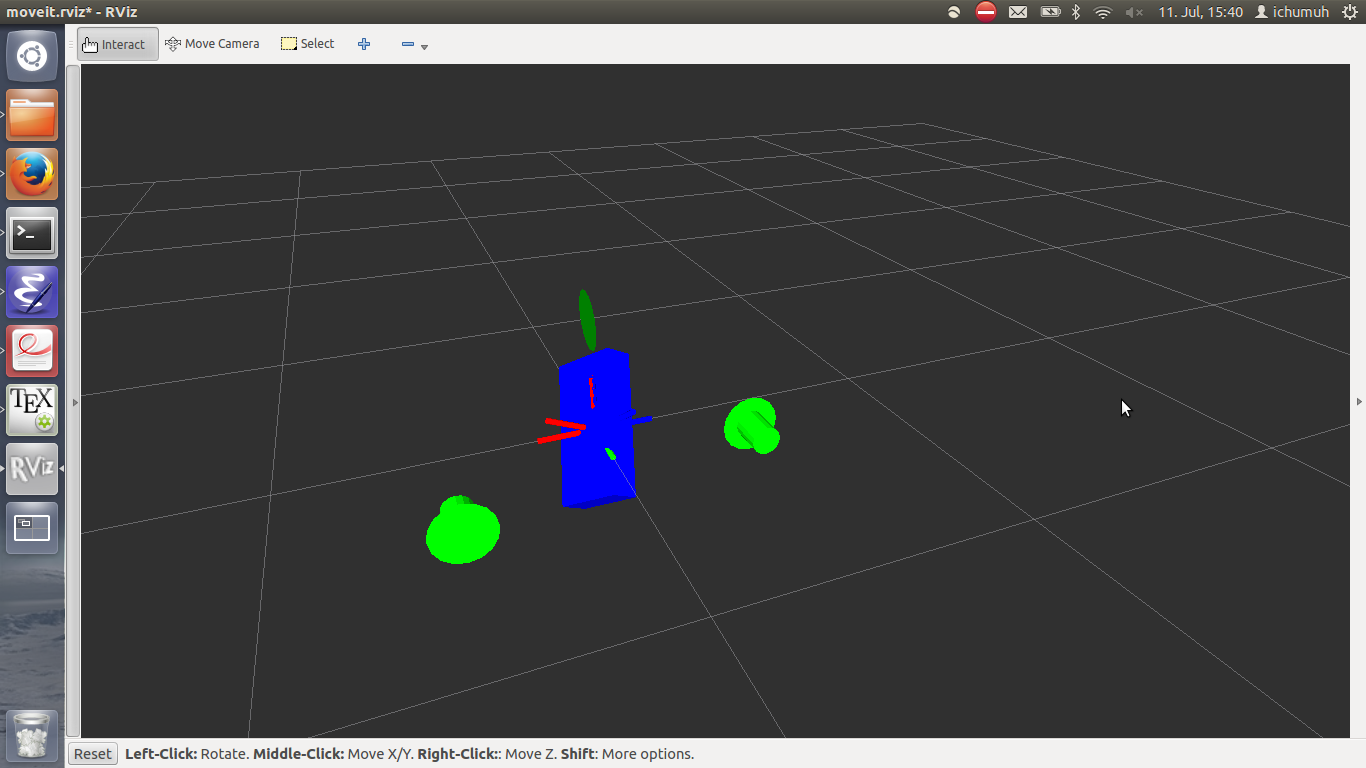
\includegraphics[width=.4\textwidth]{pictures/rviz2.png}
    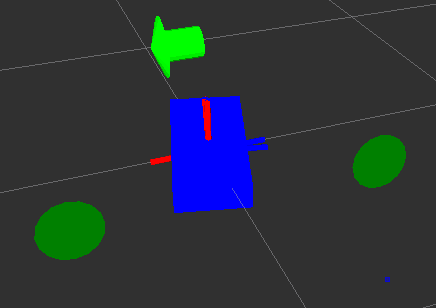
\includegraphics[width=.5\textwidth]{pictures/rviz1.png}    
  \end{center}
  \caption{Darstellung der Handydaten und Motorkommandos in Rviz}
  \label{fig:pancake}
\end{figure}

%\includegraphics[scale=1]{asd}
\begin{thebibliography}{9}

\bibitem{Code}
  Jannik Buckelo, Simon Stelter,
  \emph{Code zur Steuerung des SUTURObot v2}.
  \url{https://github.com/jannikb/nxt\_lisp}.

\end{thebibliography}

\section*{Anhang}
\includepdfset{pages=-,noautoscale}
\subsection*{Projekt "Ubersicht}
\includepdf{./project-sheet.pdf}

\end{document}








